\chapter{复数与复变函数\label{chap1}}
复变函数论讨论的是复变数的函数理论,也就是复数域上的微积分学.本章先从较高的角度帮助读者系统地复习一下有关复数的知识,再在这个基础上引进复变函数及其连续性的概念.

\section{复数的定义及其运算\label{sec1.1}}
我们把复数定义为一对有序的实数$(a,b)$, 如果用$\MR$记实数的全体,$\MC$记复数的全体,那么
\[
  \MC = \{(a,b): a\in\MR, b\in\MR \}.
\]
在这个集合中定义加法和乘法两种运算:
\begin{gather*}
  (a,b) + (c,d) = (a + c, b + d),\\
  (a,b)(c,d) = (ac - bd, ad + bc).
\end{gather*}
容易验证,加法和乘法都满足交换律和结合律;$(0,0)$是零元素,
$(-a,-b)$是$(a,b)$的负元素;$(1,0)$是乘法的单位元素;每个非零元素$(a,b)$有逆元素$\bigg(\frac a{a^2+b^2},-\frac b{a^2+b^2}\bigg)$;此外,$\MC$中的加法和乘法还满足分配律:
\[
  [(a,b) + (c,d)](e,f) = (a,b)(e,f) + (c,d)(e,f).
\]
因此,$\MC$在上面定义的加法和乘法运算下构成一个域,称为\textbf{复数域}\index{F!复数域}. 如果记
\[
  \widetilde{\MR} = \{(a,0): a\in\MR \},
\]
那么$\widetilde{\MR}$是$\MC$的一个子域. 显然,$(a,0)\to a$是$\widetilde{\MR}$与$\MR$之间的一个同构对应,因此,实数域$\MR$是$\MC$的一个子域.我们直接记$(a,0)=a$. 在$\MC$中,$(0,1)$这个元素有其特殊性,它满足
\[
  (0,1)^2 = (0,1)(0,1) = (-1,0) = -1.
\]
专门用$\ii$记$(0,1)$这个元素,于是有$\ii^2=-1$.由于$(0,b)=(b,0)\cdot(0,1)=b\ii$,于是每一个复数$(a,b)$都可写成
\[
  (a,b) = (a,0) + (0,b) = a + b\ii.
\]

复数域和实数域的一个重要区别是在复数域中不能定义两个复数的大小.为了证明这一事实,我们先给出有序域的概念.

\begin{definition}\label{def1.1.1}
域$\MF$称为\textbf{有序域}\index{Y!域!有序域},如果在$\MF$的元素间能确定一种关系(记为$a<b$),其满足下列要求:
\begin{eenum}
  \item \label{def1.1.1.1}对$\MF$中任意两个元素$a,b$, 下述三个关系中必有而且只有一个成立:
    \[
      a < b, \quad a = b,\quad b < a;
    \]
  \item \label{def1.1.1.2}如果$a<b,b<c$,那么$a<c$;
  \item \label{def1.1.1.3}如果$a<b$,那么对任意$c$,有$a+c<b+c$;
  \item \label{def1.1.1.4}如果$a<b,c>0$,那么$ac<bc$.
\end{eenum}
\end{definition}
容易知道,实数域是有序域,而复数域则不是.
\begin{theorem}\label{thm1.1.2}
  复数域不是有序域.
\end{theorem}
\begin{proof}
  如果$\MC$是有序域,那么因为$\ii\ne0$, $\ii$与$0$之间必有$\ii>0$或$\ii<0$的关系.如果$\ii>0$, 则由 \ref{def1.1.1.4} 得$\ii\cdot\ii>\ii\cdot0$, 即$-1>0$,再由 \ref{def1.1.1.3}, 两端都加$1$,即得$0>1$.另一方面,从$-1>0$还可得$-1\cdot(-1)>0\cdot(-1)$,即$1>0$,这和刚才得到的$0>1$矛盾.如果$\ii<0$,两端都加$-\ii$,再由 \ref{def1.1.1.4},两端乘$-\ii$,得$-1>0$.重复上面的讨论,即可得$0>-1$和$0<-1$的矛盾.所以,复数域不是有序域.
\end{proof}

从现在开始,我们不再用实数对$(a,b)$来记复数,而直接用$z=a+b\ii$记复数,$a$称为$z$的\textbf{实部}\index{F!复数!实部},$b$称为$z$的\textbf{虚部}\index{F!复数!虚部},分别记为$a=\Re z,b=\Im z$.加法和乘法用现在的记号定义为:
\begin{align*}
  & (a + b\ii) + (c + d\ii) = (a + c) + (b + d)\ii,\\
  & (a + b\ii) (c + d\ii) = (ac - bd) + (ad + bc)\ii.
\end{align*}
减法和除法分别定义为加法和乘法的逆运算:
\begin{align*}
  & (a + b\ii) - (c + d\ii) = (a - c) + (b - d)\ii,\\
  & \frac{a + b\ii}{c + d\ii} = (a + b\ii)\bigg(\frac{c - d\ii}{c^2 + d^2}\bigg)
  = \frac{ac + bd}{c^2 + d^2} + \frac{bc - ad}{c^2 + d^2}\ii.
\end{align*}

设$z=a+b\ii$是一复数,定义
\begin{align*}
  & |z| = \sqrt{a^2+b^2},\\
  & \bar z = a-b\ii,
\end{align*}
$|z|$称为$z$的\textbf{模}\index{F!复数!模}或绝对值,$\bar z$称为$z$的\textbf{共轭复数}\index{F!复数!共轭复数}.下面是它们的一些基本性质:
\begin{prop}\label{prop1.1.3}
  设$z$和$w$是两个复数,那么
  \begin{eenum}
    \item $\Re z=\frac12(z+\bar z),\Im z=\frac1{2\ii}(z-\bar z)$;\label{prop1.1.3.1}
    \item $z\bar z=|z|^2$;\label{prop1.1.3.2}
    \item $\overline{z+w}=\bar z+\bar w,\overline{zw}=\bar z\bar w$;\label{prop1.1.3.3}
    \item $|zw|=|z|\,|w|,\left|\frac zw\right|=\frac{|z|}{|w|}$;\label{prop1.1.3.4}
    \item $|z|=|\bar z|$.\label{prop1.1.3.5}
  \end{eenum}
\end{prop}

这些性质的证明都很简单,但在证明 \ref{prop1.1.3.4} 时,初学者往往会用$z$和$w$的实部和虚部来表示$|zw|$和$|z|\,|w|$,从而证明它们相等. 其实,利用 \ref{prop1.1.3.2} 来证明要简单得多:
\[
  |zw|^2 = (zw)(\overline{zw}) = |z|^2|w|^2.
\]

\begin{prop}\label{prop1.1.4}
  设$z$和$w$是两个复数,那么
  \begin{eenum}
    \item $|\Re z|\le |z|,|\Im z|\le |z|$;\label{prop1.1.4.1}
    \item $|z+w|\le|z|+|w|$,等号成立当且仅当存在某个$t\ge0$,使得$z=tw$;\label{prop1.1.4.2}
    \item $|z-w|\ge\bigl||z|-|w|\bigr|$.\label{prop1.1.4.3}
  \end{eenum}
\end{prop}
\begin{proof}
(1) 从$\Re z,\Im z$和$|z|$的定义马上知道不等式成立.

(2) 利用命题 \ref{prop1.1.3} 的 \ref{prop1.1.3.2},\ref{prop1.1.3.1} 和这里的不等式 \ref{prop1.1.4.1},即得
\begin{align*}
  |z+w|^2 & = (z+w)(\overline{z + w}) = |z|^2+2\Re(z\bar w) + |w|^2\\
  &\le|z|^2 + 2|z|\,|w| + |w|^2 = \big(|z| + |w|\big)^2,
\end{align*}
由此即知 \ref{prop1.1.4.2} 成立.由上面的不等式可以看出,等式成立的充要条件是$\Re(z\bar w)=|z\bar w|$,这等价于$z\bar w\ge0$.不妨设$w\ne0$($w=0$时,等号显然成立),由于$\bar w=\frac{|w|^2}{w}$,上面的不等式等价于$\frac zw|w|^2\ge0$. 令$t=\left(\frac zw|w|^2\right)\frac1{|w|^2}$,则$t\ge0$,而且$z=tw$.

(3) 是 \ref{prop1.1.4.2} 的简单推论,证明留给读者作练习.
\end{proof}

设$z_1,\cdots,z_n$是任意$n$个复数,用数学归纳法,容易得到不等式
\[
  |z_1 + \cdots + z_n| \le |z_1| + \cdots + |z_n|.
\]
请读者给出上述不等式中等号成立的条件.

\begin{xiti}
  \item 证明命题 \ref{prop1.1.3} 中的 \ref{prop1.1.3.1}, \ref{prop1.1.3.2}, \ref{prop1.1.3.3}, \ref{prop1.1.3.5}.
  \item 设$z_1,\cdots,z_n$是任意$n$个复数,证明:
    \[
      |z_1 + \cdots + z_n | \le |z_1| + \cdots + |z_n|,
    \]
    并给出不等式中等号成立的条件.
  \item 证明:
    \[
      \frac1{\sqrt2} \bigl(|\Re z| + |\Im z|\bigr) \le |z| \le |\Re z| + |\Im z|.
    \]
  \item 若$|z_1|=\lambda|z_2|,\lambda>0$,证明:
    \[
      |z_1 - \lambda^2z_2| = \lambda|z_1 - z_2|.
    \]
  \item 设$|a|<1$,证明: 若$|z|=1$,则
    \[
      \bigg| \frac{z-a}{1-\bar az} \bigg| = 1.
    \]
  \item 设$|a|<1,|z|<1$,证明:
    \begin{enuma}
      \item $\bigg|\frac{z-a}{1-\bar az}\bigg|<1$;
      \item $1-\bigg|\frac{z-a}{1-\bar az}\bigg|^2=\frac{\bigl(1-|a|^2\bigr)\bigl(1-|z|^2\bigr)}{|1-\bar az|^2}$;
      \item $\frac{\bigl||z|-|a|\bigr|}{1-|a|\,|z|}\le\bigg|\frac{z-a}{1-\bar az}\bigg|\le
        \frac{|z|+|a|}{1+|a|\,|z|}$.
    \end{enuma}
  \item 设$z_1,\cdots,z_n,w_1,\cdots,w_n$是任意$2n$个复数,证明复数形式的\textbf{Lagrange等式}:\index{L!Lagrange等式}
    \[
      \bigg| \sum_{j=1}^n{z_jw_j} \bigg|^2=\bigg( \sum_{j=1}^n{| z_j |^2} \bigg) \bigg( \sum_{j=1}^n{| w_j |^2} \bigg) -\sum_{1\leqslant j<k\leqslant n}{\left| z_j\bar{w}_k-z_k\bar{w}_j \right|^2},
    \]
    并由此推出\textbf{Cauchy不等式}:\index{B!不等式!Cauchy不等式}
    \[
      \bigg| \sum_{j=1}^n{z_jw_j} \bigg|^2\leqslant \bigg( \sum_{j=1}^n{| z_j |^2} \bigg) \bigg( \sum_{j=1}^n{| w_j |^2} \bigg).
    \]
    不等式中等号成立的条件是什么?
  \item 设$z_1,\cdots,z_n$是任意$n$个复数,证明必有$\{1,2,\cdots,n\}$的子集$E$,使得
    \[
      \bigg| \sum_{j\in E}{z_j} \bigg|\geqslant \frac{1}{6}\sum_{j=1}^n{\left| z_j \right|}.
    \]

\end{xiti}

\section{复数的几何表示\label{sec1.2}}
在平面上取定一个直角坐标系,实数对$(a,b)$就表示平面上的一个点,所以复数$z=a+b\ii$可以看成平面上以$a$为横坐标、以$b$为纵坐标的一个点(图 \ref{fig1.1}).这个点的极坐标设为$(r,\theta)$,那么
\begin{figure}[!ht]
  \centering
  \begin{tikzpicture}[> = Stealth,scale = 0.8,thick]
    \draw [->] (-1,0) -- (0,0)node[below left]{$O$} -- (7,0)node[below]{$x$};
    \draw [->] (0,-1) -- (0,5.4)node[right]{$y$};
    \draw (0,0) -- node[above]{$r$}(5,3.5) node[above]{$(a,b)$} -- node[right]{$b$}(5,0)
      --node[below]{$a$}cycle;
    \draw (0.5,0) arc (0:34:0.5);
    \node at (18:0.8) {$\theta$};
  \end{tikzpicture}
  \caption{}\label{fig1.1}
\end{figure}
\[
  a = r\cos\theta,\quad b = r\sin\theta,
\]
因而复数$z=a+b\ii$也可表示为
\[
  z = r(\cos\theta + \ii\sin\theta).
\]
这里, $r=|z|=\sqrt{a^2+b^2}$就是前面定义过的$z$的模, $\theta$称为$z$的\textbf{辐角}\index{F!复数!辐角},记为$\theta=\Arg z$.容易看出,如果$\theta$是$z$的辐角,那么$\theta+2k\pi$也是$z$的辐角,这里,$k$是任意的整数,因此$z$的辐角有无穷多个.但在$\Arg z$中,只有一个 $\theta$ 满足$-\pi<\theta\le\pi$,称这个$\theta$为$z$的\textbf{辐角的主值}\index{F!复数!辐角主值},把它记为$\arg z$.因而
\[
  \Arg z = \arg z + 2k\pi,\quad k\in\MZ,
\]
这里, $\MZ$表示整数的全体. 注意, $0$的辐角没有意义.

我们还可把复数$z=a+b\ii$看成在$x$轴和$y$轴上的投影分别为$a$和$b$的一个向量,这时我们就把复数和向量作为同义语来使用.容易知道,由一向量经过平行移动所得的所有向量表示的是同一个复数.如果一个向量的起点和终点分别为复数$z_1$和$z_2$,那么这个向量所表示的复数便是$z_2-z_1$,因而$|z_2-z_1|$就表示$z_1$与$z_2$之间的距离.特别地,当一个向量的起点为原点时,它的终点所表示的复数和向量所表示的复数是一致的.

\noindent\begin{minipage}{0.4\textwidth}
  \centering
  \begin{tikzpicture}[> = Stealth, thick, scale = 0.7]
    \draw [->] (-1,0) -- (0,0)node[below left]{$O$} -- (5,0)node[below]{$x$};
    \draw [->] (0,-0.6) -- (0,5)node[right]{$y$};
    \draw [-{Stealth[width=3pt]}] (0,0) -- (1.4,3)coordinate(A) node[above left]{$z_2$};
    \draw [-{Stealth[width=3pt]}] (0,0) -- (2.8,1)coordinate(B) node[below right]{$z_1$};
    \draw [-{Stealth[width=3pt]}] (0,0) -- (4.2,4)node[above right]{$z_1+z_2$};
    \draw [densely dashed] (4.2,4) -- (1.4,3) (4.2,4) -- (2.8,1);
    \draw [-{Stealth[width=3pt]}] (A) -- node[above right,pos=0.8]{$z_1-z_2$} (B);
  \end{tikzpicture}
  \captionof{figure}{\label{fig1.2}}
\end{minipage}
\begin{minipage}{0.6\textwidth}\parindent=2em
  由此可以知道,前面定义的复数的加法和向量的加法是一致的:把两个不重合的非零向量$z_1$和$z_2$的起点取在原点,以$z_1$和$z_2$为两边作平行四边形,那么以原点为起点沿对角线所作的向量就表示$z_1+z_2$;以$z_2$为起点,$z_1$为终点的向量就表示$z_1-z_2$(图 \ref{fig1.2}).现在再来看 \ref{sec1.1} 节命题 \ref{prop1.1.4} 中 \ref{prop1.1.4.2} 的不等式$|z_1+z_2|\le|z_1|+|z_2|$,它实际上就是三角形两边之和大于第三边的最简单的几何命题.
\end{minipage}

为了说明复数乘法的几何意义,我们采用复数的三角表示式.设
\begin{gather*}
  z_1 = r_1(\cos\theta_1 + \ii\sin\theta_1),\\
  z_2 = r_2(\cos\theta_2 + \ii\sin\theta_2),
\end{gather*}
那么
\[
  z_1z_2 = r_1r_2[\cos(\theta_1 + \theta_2) + \ii\sin(\theta_1 + \theta_2)].
\]
由此立刻得到
\begin{align*}
  & |z_1z_2| = |z_1|\,|z_2|,\\
  & \Arg(z_1z_2) = \Arg z_1 + \Arg z_2.
\end{align*}
第一个等式在 \ref{sec1.1} 节中已经证明过;第二个等式应该理解为两个集合的相等.这就是说,两个复数的乘积是这样一个复数,它的模是两个复数的模的乘积,它的辐角是两个复数的辐角之和.从几何上看,用复数$w$乘复数$z$,相当于把$z$沿反时针方向转动大小为$\arg w$的角,再让$z$的长度伸长$|w|$倍.特别地,如果$w$是单位向量,那么$w$乘$z$的结果就是把$z$沿反时针方向转动大小为$\arg w$的角.例如,已知$\ii$是单位向量,它的辐角为$\frac\pi2$,因此$\ii z$就是把$z$按反时针方向转动$\frac\pi2$角所得的向量.这种几何直观在考虑问题时非常有用.

再看复数的除法,由于
\[
  \frac{z_1}{z_2} = \frac{r_1}{r_2}[\cos(\theta_1 - \theta_2) + \ii\sin(\theta_1 - \theta_2)],
\]
所以
\begin{align*}
  & \bigg| \frac{z_1}{z_2} \bigg| = \frac{|z_1|}{|z_2|},\\
  & \Arg\bigg( \frac{z_1}{z_2} \bigg) = \Arg z_1-\Arg z_2.
\end{align*}
这里,第二个等式也理解为集合的相等.这说明向量$z_1$与$z_2$之间的夹角可以用$\Arg \bigg(\frac{z_1}{z_2}\bigg)$来表示,这一简单的事实在讨论某些几何问题时很有用.例如,用它很容易证明向量$z_1$与$z_2$垂直的充要条件是$\Re (z_1\bar z_2)=0$.这是因为$z_1$与$z_2$垂直就是$z_1$与$z_2$之间的夹角为$\pm\frac\pi2$,即$\arg \bigg(\frac{z_1}{z_2}\bigg)=\pm\frac\pi2$,这说明$\frac{z_1}{z_2}$是一个纯虚数,因而$z_1\bar z_2=\frac{z_1}{z_2}|z_2|^2$也是一个纯虚数,即$\Re(z_1\bar z_2)=0$.同样道理,可以得到$z_1$与$z_2$平行的充要条件为$\Im(z_1\bar z_2)=0$.

利用复数知识来处理几何问题,有时显得非常方便,下面是两个这方面的例子.
\begin{example}
  在图 \ref{fig1.3} 的三角形中,$AB=AC,PQ=RS,M$和$N$分别是$PR$和$QS$的中点.证明: $MN\bot BC$.
\end{example}
\begin{figure}[!ht]
  \centering
  \begin{tikzpicture}[thick]
    \tkzDefPoints{0/0/A, 5/0/B, 1.5/0/P, 3.5/0/Q}
    \coordinate(C) at (35:5);
    \coordinate(R)at(35:1.7);
    \coordinate(S)at(35:3.7);
    \tkzDefMidPoint(P,R) \tkzGetPoint{M}
    \tkzDefMidPoint(Q,S) \tkzGetPoint{N}
    \tkzInterLL(M,N)(B,C) \tkzGetPoint{D}
    \draw (A) -- (C) -- (B) -- cycle (P) -- (R) (Q) -- (S) (M) node[left=-1mm]{$M$} -- (D);
    \tkzMarkRightAngle[scale=0.5](B,D,M)
    \tkzLabelPoints[below](A,P,Q,B)
    \tkzLabelPoints[above](R,S,C)
    \node [shift={(-0.13,-0.22)}] at(N){$N$};
    \path(A) -- node[above]{$r$}(R) -- node[above]{$h$}(S)
    (A) -- node[below]{$a$}(P) -- node[below]{$h$}(Q);
    \draw (0.5,0) arc (0:35:0.5);
    \node at(20:0.7) {$\theta$};
  \end{tikzpicture}
  \caption{}\label{fig1.3}
\end{figure}
\begin{proof}
把$A$取作坐标原点,$AB$所在的直线取作$x$轴,那么$P,Q$的坐标分别为$a$和$a+h$.如果用$\ee^{\ii\theta} $记$\cos\theta+\ii\sin\theta$,那么$R$点和$S$点可分别用复数$r\ee^{\ii\theta}$和$(r+h)\ee^{\ii\theta}$表示.由于$M$和$N$分别是$PR$和$SQ$的中点,所以$M$和$N$可以分别用复数表示为
\begin{align*}
  & M: \frac12 \big( a + r\ee^{\ii\theta} \big),\\
  & N: \frac12 \big[ (a + h) + (r + h)\ee^{\ii\theta} \big].
\end{align*}
若记$z_1=\overrightarrow{MN}$,则
\[
  z_1 = \frac12 \big[ (a + h) + (r + h)\ee^{\ii\theta} \big] - \frac12 \big( a + r\ee^{\ii\theta} \big) =
  \frac h2 \big( 1 + r\ee^{\ii\theta} \big).
\]
如果记$B$的坐标为$b$,因为$AB=AC$,所以$C$的坐标为$b\ee^{\ii\theta}$. 若记$z_2=\overrightarrow{BC}$,则
\[
  z_2 = b\ee^{\ii\theta} - b = b\big( \ee^{\ii\theta} - 1 \big).
\]
现在
\[
  z_1\bar z_2 = \frac h2 \big( 1 + \ee^{\ii\theta} \big)b \big( \ee^{-\ii\theta} - 1 \big)\\
  = \frac{bh}2 \big( \ee^{-\ii\theta} - \ee^{\ii\theta} \big) = -\ii bh\sin\theta,
\]
因为$\Re(z_1\bar z_2)=0$.所以$z_1$垂直$z_2$,即$MN\bot BC$.
\end{proof}

\begin{example}
  证明:平面上四点$z_1,z_2,z_3,z_4$共圆的充要条件为
  \begin{equation}\label{eq1}
    \Im\bigg( \frac{z_1-z_3}{z_1-z_4} \bigg/ \frac{z_2-z_3}{z_2-z_4} \bigg)=0.
  \end{equation}
\end{example}
\begin{proof}
  从图 \ref{fig1.4} 可以看出,$z_1,z_2,z_3,z_4$四点共圆的充要条件是向量$z_1-z_3$和$z_1-z_4$的夹角等于向量$z_2-z_3$和$z_2-z_4$的夹角或互补(当$z_2$在$z_3$与$z_4$之间时),即
  \begin{figure}
    \centering
    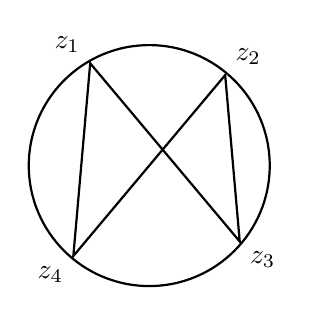
\begin{tikzpicture}[thick, scale = 1.5]
      \draw (0,0) circle (1.02);
      \draw (120:1) node[above left]{$z_1$} -- (-130:1) node[below left]{$z_4$}
        -- (50:1)node[above right]{$z_2$} -- (-40:1)node[below right]{$z_3$} -- cycle;
    \end{tikzpicture}
    \caption{\label{fig1.4}}
  \end{figure}
  \begin{align*}
    \arg\bigg( \frac{z_1-z_3}{z_1-z_4} \bigg/ \frac{z_2-z_3}{z_2-z_4} \bigg)
    & = \arg\bigg( \frac{z_1-z_3}{z_1-z_4} \bigg) - \arg\bigg( \frac{z_2-z_3}{z_2-z_4} \bigg)\\
    & = 0 \text{ 或 }\pm\pi.
  \end{align*}
  这说明复数$\frac{z_1-z_3}{z_1-z_4}\bigg/\frac{z_2-z_3}{z_2-z_4}$在实轴上,因而等式 \eqref{eq1} 成立.
\end{proof}


还有一些有趣的例子,放在习题中供读者练习.

给定复数$w$,如何计算$\sqrt[\leftroot{-1}\uproot{2} n]{w}$?也就是要求复数$z$,使得$z^n=w$.我们从de Moivre 公式说起.设
$z_1=r_1(\cos\theta_1+\ii\sin\theta_1),\cdots,z_n=r_n(\cos\theta_n+\ii\sin\theta_n)$
是给定的$n$个复数,容易用数学归纳法证明:
\[
  z_1 \cdots z_n = r_1 \cdots r_n[ \cos(\theta_1 + \cdots + \theta_n) + \ii\sin(\theta_1 + \cdots + \theta_n) ].
\]
特别当$z_1=\cdots=z_n$都是单位向量时,就有
\[
  (\cos\theta + \ii\sin\theta)^n = \cos n\theta + \ii\sin n\theta,
\]
这就是著名的 \textbf{de Moivre 公式}\index{G!公式!de Moivre 公式}. 其实对于负整数,上面的公式也成立:
\begin{align*}
  (\cos\theta + \ii\sin\theta)^{-n} & = \frac1{(\cos\theta + \ii\sin\theta)^n}
  = \frac1{\cos n\theta + \ii\sin n\theta}\\
  & = \cos n\theta - \ii\sin n\theta = \cos(-n)\theta + \ii\sin(-n)\theta.
\end{align*}

现在设$w=r(\cos\theta+\ii\sin\theta)$是给定的,要求的$z=\rho(\cos\varphi+\ii\sin\varphi)$.由 de Moivre 公式, $z^n=w$等价于
\[
  \rho^n( \cos n\varphi + \ii\sin n\varphi) = r(\cos \theta + \ii\sin\theta).
\]
由此即得$\rho=\sqrt[\leftroot{-1}\uproot{2} n]r,n\varphi=\theta+2k\pi,k=0,1,\cdots,n-1$.这就是说,共有$n$个复数满足$z^n=w$,它们是
\[
  z = \sqrt[\leftroot{-1}\uproot{2} n]{|w|}\bigg( \cos\frac{\theta + 2k\pi}n + \ii\sin\frac{\theta + 2k\pi}n \bigg), k = 0,1,\cdots,n-1.
\]
这$n$个复数恰好是以原点为中心、$\sqrt[\leftroot{-1}\uproot{2} n]{|w|}$为半径的圆的内接正$n$边形的顶点. 当$w=1$时, 若记$\omega=\cos\frac{2\pi}n+\ii\sin\frac{2\pi}n$,则$\sqrt[\leftroot{-1}\uproot{2} n]1$的$n$个值为
\[
  1,\omega,\omega^2,\cdots,\omega^{n-1},
\]
称为$n$个\textbf{单位根}\index{D!单位根}. 如果用$\sqrt[\leftroot{-1}\uproot{2} n]{w}$记$w$的任一$n$次根,那么$w$的$n$个$n$次根又可表示为
\[
  \sqrt[\leftroot{-1}\uproot{2} n]w,\sqrt[\leftroot{-1}\uproot{2} n]w\omega,\cdots,\sqrt[\leftroot{-1}\uproot{2} n]{w}\omega^{n-1}.
\]

\begin{xiti}\hypertarget{xiti1.2}{}
 \item 把复数$z=1+\cos\theta+\ii\sin\theta$写成三角形式.
 \item 问$n$取何值时有$(1+\ii)^n=(1-\ii)^n$ ?
 \item 证明:
   \[
     \sum_{k=0}^n\cos k\theta = \frac{\sin\frac\theta2 + \sin\left(n+\frac12\right)\theta}{2\sin\frac\theta2},\quad
     \sum_{k=0}^n\sin k\theta = \frac{\cos\frac\theta2 - \cos\left(n+\frac12\right)\theta}{2\sin\frac\theta2}.
   \]
 \item 证明:$\triangle z_1z_2z_3$和$\triangle w_1w_2w_3$同向相似的充分必要条件为
   \[
     \begin{vmatrix}
     z_1 & w_1 & 1 \\
     z_2 & w_2 & 1 \\
     z_3 & w_3 & 1
     \end{vmatrix}=0.
   \]
 \item 设$z_1\ne z_2$,证明:
  \begin{enuma}
    \item $z$位于以$z_1$和$z_2$为端点的开线段上,当且仅当存在$\lambda\in (0,1)$,使得
       \[
         z = \lambda z_1 + (1 - \lambda)z_2;
       \]
    \item $z$位于以$z_1$和$z_2$为端点的开圆弧上,当且仅当存在$\theta\,\big(0<|\theta|<\pi\big)$,使得
       \[
         \arg\frac{z-z_1}{z-z_2} = \theta.
       \]
  \end{enuma}
 \item 证明:三点$z_1,z_2,z_3$共线的充要条件为
   \[
     \begin{vmatrix}
       z_1 & \bar z_1 & 1 \\
       z_2 & \bar z_2 & 1 \\
       z_3 & \bar z_3 & 1
     \end{vmatrix}=0.
   \]
 \item 图 \ref{fig1.5} 是三个边长为$1$的正方形,证明:
   \[
     \angle AOD + \angle BOD + \angle COD = \frac\pi2.
   \]
 \item 图 \ref{fig1.6} 中, $ABED,ACFG$是正方形, $AH\bot BC,M$是$DG$的中点.证明: $M,A,H$三点共线.
   \begin{figure}[!ht]
     \begin{minipage}[b]{0.48\textwidth}
       \centering
       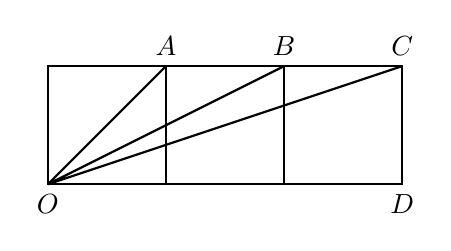
\begin{tikzpicture}[thick, scale = 1.5]
         \draw (0,0) node[below]{$O$} -- (3,0) node[below]{$D$} -- (3,1) node[above]{$C$}
          -- (2,1) node[above]{$B$} -- (1,1) node[above]{$A$} -- (0,1) -- cycle;
         \draw (0,0) -- (1,1) (0,0) -- (2,1) (0,0) -- (3,1);
         \draw (1,0) -- (1,1) (2,0) -- (2,1);
       \end{tikzpicture}
       \caption{}\label{fig1.5}
     \end{minipage}\hfill%
     \begin{minipage}[b]{0.48\textwidth}
       \centering
       \begin{tikzpicture}[thick]
         \tkzDefPoints{0/0/B, 2/0/C, 0.8/1.2/A}
         \tkzDefSquare(B,A) \tkzGetPoints{D}{E}
         \tkzDrawPolygon[thick](B,A,D,E)
         \tkzDefSquare(A,C) \tkzGetPoints{F}{G}
         \tkzDrawPolygon[thick](A,C,F,G)
         \tkzDefMidPoint(D,G) \tkzGetPoint{M}
         \tkzInterLL(M,A)(B,C)
         \tkzGetPoint{H}
         \draw (B) -- (C) (D) -- (G)(M) -- (H);
         \tkzMarkRightAngle[scale=0.5](C,H,M)
         \tkzLabelPoints[below](B,C,H)
         \tkzLabelPoints[above](D,M,G)
         \tkzLabelPoints[right](A,F)
         \tkzLabelPoints[left](E)
       \end{tikzpicture}
       \caption{}\label{fig1.6}
     \end{minipage}
   \end{figure}
   \begin{figure}[!ht]
     \centering
     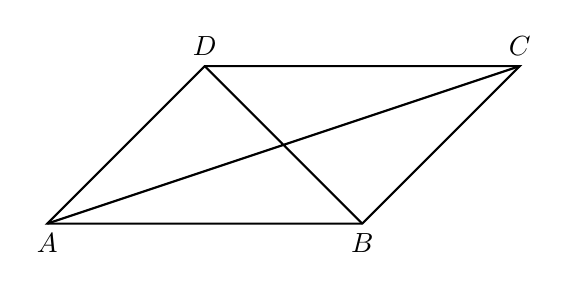
\begin{tikzpicture}[thick]
       \draw (0,0) coordinate(A) node[below]{$A$} -- ++(4,0) coordinate(B) node[below]{$B$}
       -- ++ (2,2) coordinate(C) node[above]{$C$} -- ++(-4,0) coordinate(D) node[above]{$D$}
       --cycle;
       \draw (A) -- (C) (B) -- (D);
     \end{tikzpicture}
     \caption{}\label{fig1.7}
   \end{figure}
 \item 在平行四边形$ABCD$中(见图 \ref{fig1.7}),如果
   \[
     \overline{AC}^2 \cdot \overline{BD}^2 = \overline{AB}^4 + \overline{AD}^4,
   \]
   那么这个平行四边形的锐角等于$\frac\pi4$.
 \item 证明:
   \[
     |z_1 + z_2|^2 + |z_1 - z_2|^2 = 2\big( |z_1|^2 +|z_2|^2 \big),
   \]
   并说明等式的几何意义.
 \item 设$z_1,\cdots,z_n$是单位圆周(以原点为中心、半径为$1$的圈周)上的$n$个点,如果$z_1,\cdots,z_n$是正$n$边形的$n$个顶点,证明:
     \[
       z_1 + \cdots + z_n = 0.
     \]
 \item 设$z_1,z_2,z_3$是单位圆周上的三个点,证明:这三个点是一正三角形三个顶点的充要条件为
     \[
       z_1 + z_2 + z_3 = 0.
     \]
 \item 设$z_1,z_2,z_3,z_4$是单位圆周上的四个点,证明:这四个点是一矩形顶点的充要条件为
     \[
       z_1 + z_2 + z_3 + z_4 = 0.
     \]
 \item 设$L$是由方程\hypertarget{xiti1.2.14}{}
     \[
       az\bar z + \bar\beta z + \beta\bar z + d = 0
     \]
     所确定的点的轨迹,其中$a,d$是实数, $\beta$是复数.证明:
     \begin{enuma}
       \item 当$a=0,\beta\ne0$时,$L$是直线;
       \item 当$a\ne0,|\beta|^2-ad>0$时, $L$是一圆周.并求出该圆周的圆心和半径.
     \end{enuma}
 \item \hypertarget{xiti1.2.15}{}设$z_1\ne z_2,0<\lambda\ne1$,证明由方程
     \[
       \left| \frac{z-z_1}{z-z_2} \right| = \lambda
     \]
     所确定的点$z$的轨迹是一圆周(通常称为\textbf{Apollonius圆}\index{A!Apollonius圆}),该圆周的圆心$a$和半径$R$分别为
     \[
       a = \frac{z_1-\lambda^2z_2}{1-\lambda^2}, \quad R = \frac{\lambda|z_1-z_2|}
       {|1-\lambda^2|}.
     \]
     并问$\lambda=1$时它的轨迹是什么?
 \item 如果$z_1,\cdots,z_n$都位于过原点的直线的一侧,证明$\frac1{z_1},\cdots,\frac1{z_n}$也必位于该直线的某一侧,且满足
     \[
       z_1 + \cdots + z_n \ne 0,\quad \frac1{z_1} + \cdots + \frac1{z_n} \ne 0\footnote{本题题目有误,反例可取$z_1=\ee^{\ii\frac\pi3},z_2=\ee^{\ii\frac{5\pi}6}$,直线取为$y=x$,那么$z_1,z_2$都在此直线上方,但$\frac1{z_1}$在此直线的下方,$\frac1{z_2}$在此直线的上方.}.
     \]
 \item 设$z_1,\cdots,z_n$是一个凸$n$边形的$n$个顶点,如果$a$满足关系
     \[
       \frac1{z_1-a} + \cdots + \frac1{z_n-a} = 0,
     \]
     那么$a$必在这个凸$n$边形的内部.
 \item 证明:
     \[
       \sin\frac\pi n\sin\frac{2\pi}n \cdots \sin\frac{(n-1)\pi}n = \frac n{2^{n-1}}.
     \]

     (\textbf{提示}:考虑方程式$(z+1)^n=1$的$n-1$个不为零的根的乘积.)
 \item 设$0<\theta<\frac\pi2,P_m(x)=\sum_{k=0}^m(-1)^k\binom{2m+1}{2k+1}x^{m-k}$.证明:
   \[
       \sin(2m+1)\theta = \sin^{2m+1}\theta P_m(\cot^2\theta).
   \]
 \item 利用上题结果证明:
   \begin{enuma}
     \item $\sum_{k=1}^m\cot^2\frac{k\pi}{2m+1}=\frac{m(2m-1)}3$;
     \item $\prod_{k=1}^m\cot^2\frac{k\pi}{2m+1}=\frac1{2m+1}$.
   \end{enuma}
\end{xiti}

\section{扩充平面与复数的球面表示\label{sec1.3}}
为了今后讨论的需要,我们要在$\MC$中引进一个新的数$\infty$,这个数的模是$\infty$,辐角没有意义,它和其他数的运算规则规定为:
\begin{align*}
  & z\pm\infty = \infty, \quad z\cdot \infty = \infty\,\mbox{($z\ne0$)},\\
  & \frac z{\infty}=0,\quad \frac z0 = \infty\;\mbox{($z\ne0$)};
\end{align*}
$0\cdot \infty$和$\infty\pm\infty$都不规定其意义. 引进了$\infty$的复数系记为$\MC_{\infty} $,即$\MC_{\infty}=\MC\cup\{\infty\}$.在复平面上,没有一个点和$\infty$相对应,但我们想像有一个\textbf{无穷远点}\index{F!复平面!无穷远点}和$\infty$对应,加上无穷远点的复平面称为\textbf{扩充平面}\index{F!复平面!扩充平面}或\textbf{闭平面}\index{F!复平面!闭平面},不包括无穷远点的复平面也称为\textbf{开平面}\index{F!复平面!开平面}.在复平面上,无穷远点和普通的点是不一样的,Riemann首先引进了复数的球面表示,在这种表示中,$\infty$和普通的复数没有什么区别. 设$S$是$\MR^3$中的单位球面,即
\[
  S = \{(x_1,x_2,x_3)\in\MR^3:x_1^2 + x_2^2 + x_3^2 = 1\}.
\]
把$\MC$等同于平面:
\[
  \MC = \{(x_1,x_2,0): x_1, x_2\in\MR\}.
\]
\begin{figure}[!ht]
  \centering
  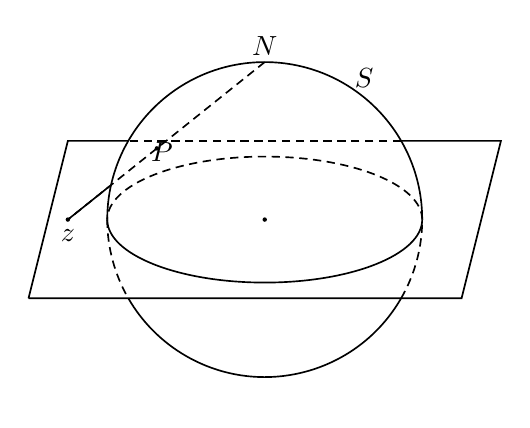
\begin{tikzpicture}[semithick]
    \draw (-3,-1 )-- ++(5.5,0) -- ++(0.5,2) -- (1.73,1)(-1.73,1) -- (-2.5,1) -- (-3,-1);
    \draw [densely dashed] (1.73,1) -- (-1.73,1);
    \fill (0,0) circle (0.8pt);
    \draw [densely dashed] (-30:2) arc (-30:0:2);
    \draw [densely dashed] (180:2) arc (180:210:2);
    \draw (-30:2) arc (-30:-150:2);
    \draw (2,0) arc (0:180:2);
    \draw [densely dashed] (2,0) arc (0:180:2 and 0.8);
    \draw (2,0) arc (0:-180:2 and 0.8);
    \node at (55:2.2) {$S$};
    \node at (0,2.2) {$N$};
    \fill (-2.5,0) coordinate(z) node[below]{$z$} circle(0.8pt);
    \draw [densely dashed] (0,2) -- (z);
    \draw (z) -- (-1.97,{-1.97*0.8+2});
    \fill (-1.37,{-1.37*0.8+2}) node[below right=-2mm] {$P$} circle(0.8pt);
  \end{tikzpicture}
  \caption{}\label{fig1.8}
\end{figure}
固定$S$的北极$N$,即$N=(0,0,1)$,对于$\MC$上的任意点$z$,联结$N$和$z$的直线必和$S$交于一点$P$(图 \ref{fig1.8}).若$|z|>1$,则$P$在北半球上;若$|z|<1$,则$P$在南半球上;若$|z|=1$,则$P$就是$z$.容易看出,当$z$趋向$\infty$时,球面上对应的点$P$趋向于北极$N$,自然地,我们就把$\MC_\infty$中的$\infty$对应于北极$N$.这样一来,$\MC_\infty$中的所有点(包括无穷远点在内)都被移植到球面上去了,而在球面上,$N$和其他的点是一视同仁的.

现在给出这种对应的具体表达式.设$z=x+\ii y$,容易算出$zN$和球面$S$的交点的坐标为
\[
  x_1 = \frac{2x}{x^2+y^2+1}, x_2 = \frac{2y}{x^2+y^2+1},x_3 = \frac{x^2+y^2-1}{x^2+y^2+1}.
\]
直接用复数$z$,可表示为
\[
  x_1 = \frac{z+\bar z}{1+|z|^2},
  x_2 = \frac{z-\bar z}{\ii\big(1+|z|^2\big)},
  x_3 = \frac{|z|^2-1}{|z|^2+1}.
\]
这样,从$z$便可算出它在球面上对应点的坐标. 反过来,从球面上的点$(x_1,x_2,x_3)$也可算出它在平面上的对应点$z$.事实上,从上面的表达式得
\[
  \left\{ \begin{aligned}
            & x_1+\ii x_2 = \frac{2z}{1+|z|^2},\\
            & 1-x_3 = \frac2{1+|z|^2},
          \end{aligned}
  \right.
\]
由此即得
\[
  z = \frac{x_1+\ii x_2}{1-x_3}.
\]
这就是所需的计算公式.

\begin{xiti}
  \item 证明:在复数的球面表示下,$z$和$\frac 1{\bar z}$的球面像关于复平面对称.
  \item 证明:在复数的球面表示下,$z$和$w$的球面像是直径对点当且仅当$z\bar w=-1$.
  \item 证明:在复数的球面表示下,$\MC_\infty$中的点$z$和$w$的球面像间的距离为
     \[\frac{2|z-w|}{\sqrt{\big(|z|^2+1\big)\big(|w|^2+1\big)}}.\]
  \item 证明:在复数的球面表示下,若$\begin{pmatrix}
  a&b\\c&d
  \end{pmatrix}$是二阶酉方阵,则$\MC_\infty$的变换$w=\frac{az+b}{cz+d}$诱导了球面绕球心的一个旋转.
  \item 证明:在复数的球面表示下,球面上的圆周对应于复平面上的圆周或直线,反之亦然.
  \item 证明:在复数的球面表示下,复平面上两条光滑曲线在交点处的夹角与它们的球面像在交点处的夹角相等.
\end{xiti}

\section{复数列的极限\label{sec1.4}}
复变函数是定义在平面点集上的复值函数,在讨论复变函数之前,必须对平面点集的知识有足够的了解.我们从复数列的极限谈起.

我们说$\MC$中的复数列$\{z_n\}$收敛到$\MC$中的点$z_0$,是指对于任给的$\varepsilon>0$,存在正整数$N$,当$n>N$时,$|z_n-z_0|<\varepsilon$,记作$\lim_{n\to\infty}z_n=z_0$.
我们称复数列$\{z_n\}$收敛到$\infty$,是指对任给的正数$M>0$,存在正整数$N$,当$n>N$时,$|z_n|>M$,记为$\lim_{n\to\infty}z_n=\infty$.

对于$a\in\MC,r>0$,称
\[B(a,r)=\{z\in\MC:|z-a|<r\}\]
为以$a$为中心、以$r$为半径的\textbf{圆盘}\index{L!邻域!圆盘}.特别当$a=0,r=1$时, $B(0,1)=\{z:|z|<1\}$称为\textbf{单位圆盘}\index{L!邻域!单位圆盘}. $B(a,r)$也称为$a$点的一个\textbf{$r$邻域},或简称为$a$的\textbf{邻域}\index{L!邻域}. 无穷远点$z=\infty$的邻域是指集合$\{z\in\MC:|z|>R\}$,记为$B(\infty,R)$.

这样,从几何上来说,$\lim_{n\to\infty}z_n=z_0$可以说成对任给的$\varepsilon>0$,当$n$充分大时,$z_n\in B(z_0,\varepsilon)$;$\lim_{n\to\infty}z_n=\infty$可以说成对任给的$M>0$,当$n$充分大时,$z_n\in B(\infty,M)$.

设$z_n=x_n+\ii y_n,z_0=x_0+\ii y_0$,从等式
\[
  |z_n - z_0| = \sqrt{(x_n-x_0)^2 + (y_n-y_0)^2}
\]
马上可以得到:$\lim_{n\to\infty}z_n=z_0$的充分必要条件是$\{z_n\}$的实部和虚部分别有$\lim_{n\to\infty}x_n=x_0$和$\lim_{n\to\infty}y_n=y_0$.

复数列$\{z_n\}$称为\textbf{Cauchy列}\index{C!Cauchy列},如果对任给的$\varepsilon>0$,存在正整数$N$,当$m,n>N$时,有$|z_n-z_m|<\varepsilon$.设$z_n=x_n+\ii y_n,z_m=x_m+\ii y_m$,那么从等式
\[
  |z_n-z_m| = \sqrt{(x_n-x_m)^2+(y_n-y_m)^2}
\]
知道,$\{z_n\}$是Cauchy列的充分必要条件是它的实部$\{x_n\}$和虚部
$\{y_n\}$都是实的Cauchy列,因而从实数域中的Cauchy收敛准则立刻得到复数域的\textbf{Cauchy收敛准则}\index{C!Cauchy收敛准则}:$\{z_n\}$收敛的充要条件是$\{z_n\}$为Cauchy列.由此知道$\MC$是\textbf{完备}\index{W!完备}的.

\begin{xiti}
  \item 设$z_0\notin(-\infty,0],z_n\ne0,\forall n\in\MN$.证明:复数列$\{z_n\}$收敛到$z_0$的充要条件是$\lim_{n\to\infty}|z_n|=|z_0|$和$\lim_{n\to\infty}\arg z_n=\arg z_0$.
  \item 设$z=x+\ii y\in\MC$,证明:
     \[
       \lim_{n\to\infty} \bigg( 1+\frac zn \bigg)^n = \ee^x(\cos y + \ii\sin y).
     \]
  \item 证明:如果$\lim_{n\to\infty}z_n=z_0$,则
     \[
       \lim_{n\to\infty} \frac{z_1 + z_2 + \cdots + z_n}n = z_0.
     \]
  \item 证明:若$\lim_{n\to\infty}z_n=z_0,\lim_{n\to\infty}w_n=w_0$,则
     \[
       \lim_{n\to\infty} \frac1n\sum_{k=1}^nz_kw_{n-k} = z_0w_0.
     \]
  \item 设无穷三角阵
     \[
       \begin{matrix}
         a_{11} &\\
         a_{21} & a_{22}\\
         a_{31} & a_{32} & a_{33}\\
         \cdots & \cdots & \cdots
       \end{matrix}
     \]
  满足
  \begin{enuma}
    \item 对任意固定的$k$,$\lim_{n\to\infty}a_{nk}=a_k$存在;
    \item $\lim_{n\to\infty}\sum_{k=1}^na_{nk}$存在;
    \item $\sum_{k=1}^n|a_{nk}|\le M<\infty,\forall n\in \MN$.
  \end{enuma}
  证明:若复数列$\{z_n\}$收敛,则$\lim_{n\to\infty}\sum_{k=1}^na_{nk}z_k$存在.
\end{xiti}

\section{开集、闭集和紧集\label{sec1.5}}
设$E$是一平面点集,$\MC$中的点对$E$而言可以分为三类:(1)如果存在$r>0$,使得$B(a,r)\subset E$,就称$a$为$E$的\textbf{内点}\index{J!集!内点};(2)如果存在$r>0$,使得$B(a,r)\subset E^{\mathrm c}$,就称$a$为$E$的\textbf{外点}\index{J!集!外点},这里,$E^{\mathrm c}$是由所有不属于$E$的点构成的集,称为$E$的\textbf{余集}\index{J!集!余集}或\textbf{补集}\index{J!集!补集};(3)如果对任意$r>
0$,$B(a,r)$中既有$E$的点,也有$E^{\mathrm c}$的点,就称$a$为$E$的\textbf{边界点}\index{J!集!边界点}. $E$的内点的全体称为$E$的\textbf{内部}\index{J!集!内部},记为$E^\circ$;$E$的外点的全体称为$E$的\textbf{外部}\index{J!集!外部},它就是$E$的余集$E^{\mathrm c}$的内部,即$(E^{\mathrm c})^\circ$;$E$的边界点的全体称为$E$的\textbf{边界}\index{J!集!边界},记为$\partial E$.

由上面的定义可知,集$E$把复平面分成三个互不相交的部分:$\MC=E^\circ\cup(E^{\mathrm c})^\circ\cup\partial E$,即
\begin{equation}\label{eq1.5.1}
  (\partial E)^{\mathrm c} = E^\circ\cup(E^{\mathrm c})^\circ.
\end{equation}

例如,$B(a,r)$中的所有点都是它的内点,即$B(a,r)=\big(B(a,r)\bigr)^\circ$,$B(a,r)$的边界$\partial B=\{z:|z-a|=r\}$,即是圆周,满足条件$|z-a|>r$的点$z$都是$B(a,r)$的外点.

如果$E$的所有点都是它的内点,即$E=E^\circ$,就称$E$为\textbf{开集}\index{J!集!开集}.如果$E^{\mathrm c}$是开集,就称$E$为\textbf{闭集}\index{J!集!闭集}.

例如,$B(a,r)$是开集,闭圆盘$\{z:|z-a|\le r\}$是闭集,$B(a,r)$和它的上半圆周的并集既不是开集也不是闭集.

点$a$称为集$E$的\textbf{极限点}\index{J!集!极限点}或\textbf{聚点}\index{J!集!聚点},如果对任意$r>0$,$B(a,r)$中除$a$外总有$E$中的点. 集$E$的所有极限点构成的集称为$E$的\textbf{导集}\index{J!集!导集},记为$E'$. $E$中不属于$E'$的点称为$E$的\textbf{孤立点}\index{J!集!孤立点}. $E$和它的导集$E'$的并称为$E$的\textbf{闭包}\index{J!集!闭包},记为$\bar E$,即$\bar E=E\cup E'$.

这些集之间有下面的关系:
\begin{prop}\label{prop1.5.1}
  对于任意集$E$,有
  \begin{eenum}
    \item $a\in\bar E$的充要条件是对任意$\varepsilon>0$,有\label{prop1.5.1.1}
    \begin{equation}\label{eq1.5.2}
       B(a,r)\cap E\ne\varnothing,
    \end{equation}
    这里,$\varnothing$表示空集;
    \item $(\bar E)^{\mathrm c}=(E^{\mathrm c})^\circ,\bar {E^{\mathrm c}}=(E^\circ)^{\mathrm c}$.\label{prop1.5.1.2}
  \end{eenum}
\end{prop}
\begin{proof}
(1) 若$a\in\bar E$,则$a\in E$或$a\in E'$,不论何者发生,总有$B(a,r)\cap E\ne\varnothing$.反之,若等式 \eqref{eq1.5.2} 成立,这说明$a$或是$E$的极限点,或是$E$的孤立点,因而$a\in\bar E$.

(2) 由 \ref{prop1.5.1.1} 知,$a\in(\bar E)^{\mathrm c}$当且仅当存在$\varepsilon>0$,使得$B(a,r)\cap E=\varnothing$,这说明$a$是$E^{\mathrm c}$的内点,即$a\in (E^{\mathrm c})^\circ$,因而$(\bar E)^{\mathrm c}=(E^{\mathrm c})^\circ$.再看第二个等式,$a\in (E^\circ)^{\mathrm c}$意味着$a$不是$E$的内点,即$a$是$E$的外点或边界点,因而对任意$\varepsilon>0$,总有$B(a,r)\cap E^{\mathrm c}\ne\varnothing$,由 \ref{prop1.5.1.1} 知$a\in \bar{E^{\mathrm c}}$. 因而$\bar {E^{\mathrm c}}=(E^\circ)^{\mathrm c}$.
\end{proof}

\begin{prop}\label{prop1.5.2}
  (1) \hypertarget{prop1.5.2.1}{}$E^\circ$是开集,$\partial E$和$\bar E$是闭集;\par
  (2) \hypertarget{prop1.5.2.2}{}$E$是闭集的充要条件是$E=\bar E$;\par
  (3) \hypertarget{prop1.5.2.3}{}$E$是闭集的充要条件是$E'\subset E$.
\end{prop}
\begin{proof}
  (1) 任取$a\in E^\circ$,则由定义知道,存在$\varepsilon>0$,使得$B(a,\varepsilon)\subset E$.显然,$B(a,\varepsilon)$中的每一点都是$E$的内点,因而$B(a,\varepsilon)\subset E^\circ$,即$a$是$E^\circ$的内点.由于$a$是任意取的,所以$E^\circ$是开集.由刚才所证,$E^\circ$和$(E^{\mathrm c})^\circ$都是开集,两个开集的并当然也是开集,由等式 \eqref{eq1.5.1} 知$(\partial E)^{\mathrm c}$是开集,因而$E$是闭集.由于$(E^{\mathrm c})^\circ$是开集,由命题 \ref{prop1.5.1} 的 \ref{prop1.5.1.2}  知,$(\bar E)^{\mathrm c}$是开集,所以$\bar E$是闭集.
  \par
  (2)如果$E=\bar E$,则由(1)知$\bar E$是闭集,所以$E$是闭集.反之,如果$E$是闭集,那么$E^{\mathrm c}$是开集,因而$E^{\mathrm c}=(E^{\mathrm c})^\circ$.另外,由命题 \ref{prop1.5.1} 的 \ref{prop1.5.1.2} 得$(\bar E)^{\mathrm c}=(E^{\mathrm c})^\circ$,因而$E^{\mathrm c}=(\bar E)^{\mathrm c}$,即$E=\bar E$.
  \par
  (3) 从 \hyperlink{prop1.5.2.2}{(2)} 立刻可得.
\end{proof}

下面给出闭集的一个重要性质,为此先定义点集$E$的直径的概念.点集$E$的\textbf{直径}\index{J!集!直径}定义为$E$中任意两点间距离的上确界,记为$\diam E$,即
\[
  \diam E = \sup\{ |z_1 - z_2|: z_1,z_2\in E \}.
\]

\begin{theorem}[(\textbf{Cantor})]\index{D!定理!Cantor定理}\label{thm1.5.3}
  若非空闭集序列$\{F_n\}$满足
  \begin{eenum}
    \item \label{thm1.5.3.1} $F_1\supset F_2\supset\cdots\supset F_n\supset\cdots$;
    \item \label{thm1.5.3.2} $\diam F_n\to 0$(当$n\to\infty$时),
  \end{eenum}
  那么$\bigcap_{n=1}^\infty F_n$是一个独点集.
\end{theorem}
\begin{proof}
  在每一个$F_n$中任取一点$z_n$,我们证明$\{z_n\}$是一个Cauchy点列.由于$\lim_{n\to\infty}\diam F_n$ $=0$,所以对任意$\varepsilon>0$,可取充分大的$N$,使得 $\diam F_N<\varepsilon$.今取$m,n>N$,由条件 \ref{thm1.5.3.1},$z_m,z_n\in F_N$,所以$|z_n-z_m|\le\diam F_N<\varepsilon$.因而$\{z_n\}$是一Cauchy序列,设其收敛于$z_0$.我们证明$z_0\in\bigcap_{n=1}^\infty F_n$.事实上,任取$F_k$,则当$n>k$时,$z_n$便全部落入$F_k$中,因为$F_k$是闭的,由命题 \ref{prop1.5.2} 的 \hyperlink{prop1.5.2.3}{(3)},$\{z_n\}$的极限$z_0\in F_k$,所以$z_0\in\bigcap_{n=1}^\infty F_n$.如果还有另一点$z_1$也属于$\bigcap_{n=1}^\infty F_n$,那么必有$|z_0-z_1|\le\diam F_n\to0$($n\to\infty$),因而$z_1=z_0$.
\end{proof}

这个定理是实数域中的区间套定理在复数域中的推广.

下面引进一类重要的集——紧集.

设$E$是一个集,$\mathscr F=\{G\}$是一个\textbf{开集族}\index{J!集!开集族},即$\mathscr F$中的每一个元素都是开集.如果$E$中每一点至少属于$\mathscr F$中的一个开集,就说$\mathscr F$是$E$的一个\textbf{开覆盖}\index{J!集!开覆盖}.

例如,$E$是任一点集,$\varepsilon$是一个给定的正数,那么
\[
  \mathscr F = \{ B(a,\varepsilon):a\in E \}
\]
便是$E$的一个开覆盖.

我们说点集$E$具有\textbf{有限覆盖性质}\index{J!集!有限覆盖性质},是指从$E$的任一个开覆盖中必能选出有限个开集$G_1,\cdots,G_n$,使得这有限个开集的并就能覆盖$E$,即
\[
  E \subset \bigcup_{j=1}^n G_j.
\]
\begin{definition}\label{def1.5.4}
  具有有限覆盖性质的集称为\textbf{紧集}\index{J!集!紧集}.
\end{definition}

例如,空集和有限集都是紧集,但单位圆盘$B(0,1)=\{z\in\MC:|z|<1\}$却不是紧集,因为
\[
  G_n = \left\{z:|z| < 1 - \frac1n\right\}, n = 2,3,\cdots,
\]
这一串同心圆构成$B(0,1)$的一个开覆盖,但从中找不出有限个集覆盖$B(0,1)$.

我们希望能找到紧集的特征.

集$E$称为是\textbf{有界}的,如果存在$R>0$,使得$E\subset B(0,R)$.
\begin{theorem}[(\textbf{Heine--Borel})]\index{D!定理!Heine--Borel定理}\label{thm1.5.5}
  在$\MC$中,$E$是紧集的充要条件为$E$是有界闭集;在$\MC_\infty$中,$E$是紧集的充要条件为$E$是闭集.
\end{theorem}
\begin{proof}
  我们先证明,如果$E$是$\MC_\infty$中的闭集或$\MC$中的有界闭集,那么$E$是紧集,即从$E$的任一开覆盖$\mathscr F$中,可以选出有限个开集覆盖$E$.先设$E$是$\MC_\infty$中的闭集,如果$z=\infty\notin E$,则因$E$是闭集,有$E=\bar E$,即$\infty\notin\bar E$,由命题 \ref{prop1.5.1} 的 \ref{prop1.5.1.1},存在$R>0$,使得$B(\infty,R)\cap E=\varnothing$,即$E\subset\overline{B(0,R)}$,因而$E$是有界闭集.如果$z=\infty\in E$,由开覆盖的定义,$\infty$属于$\mathscr F$中的某一个开集,而$E$在这个开集之外的部分是一有界闭集.总之,不论何种情况发生,只要考虑$E$是有界闭集的情形就够了.

  现设$E$是有界闭集,如果它不是紧集,那么从$E$的开覆盖$\mathscr F$中不能取出有限个开集来覆盖$E$.因为$E$是有界的,它一定包含在一个充分大的闭正方形$Q$中:
  \[
    Q = \{(x,y): |x| \le M,|y| \le M\}.
  \]
  把这个正方形分成相等的四个小正方形,则其中必有一个小正方形$Q_1$,使得$Q_1\cap E$是有界闭集且不具有有限覆盖性质.再把$Q_1$分成四个相等的小正方形,其中必有一个小正方形$Q_2$具有上述同样的性质.这个过程可以无限地进行下去,得到一列闭正方形$\{Q_n\}$.如果记$F_n=Q_n\cap E$,那么$F_n$满足下列条件:
  \begin{eenum}
    \item  \label{thm1.5.5.1}$F_n$是有界闭集;
    \item  \label{thm1.5.5.2}$F_n\supset F_{n+1},n=1,2,\cdots$;
    \item  \label{thm1.5.5.3}不能从$\mathscr F$中取出有限个开集来覆盖$F_n$;
    \item  \label{thm1.5.5.4}当$n\to\infty$时,$\diam F_n\le\frac M{2^n}\sqrt2\to0$.
  \end{eenum}
  由 \ref{thm1.5.5.1}, \ref{thm1.5.5.2}, \ref{thm1.5.5.4}知道$\{F_n\}$满足Cantor定理的条件,因而存在复数$z_0$,使得$\bigcap_{n=1}^\infty F_n=\{z_0\}$.由于$z_0\in F_n\subset E$,故在$\mathscr F$中必有一个开集$G_0$,使得$z_0\in G_0$.由于$z_0$是$G_0$的内点,故有$z_0$的邻域$B(z_0,\varepsilon)\subset G_0$.由于$\diam F_n\to0$,故当$n$充分大时, $F_n\subset B(z_0,\varepsilon)\subset G_0$,这就是说$G_0$覆盖了$F_n$,这与 \ref{thm1.5.5.3} 矛盾. 因此$E$是紧集.

  现在证明必要性.只要对扩充平面的情形来证明就够了,因为如果一个集对扩充平面是闭的,它又不包含无穷远点,那么它必然是有界的.设$E$是一个紧集,我们要证明它是闭集,只要证明$E^c$是开集即可.为此,任取$a\in E^{\mathrm c}$,只要证明$a$是$E^{\mathrm c}$的内点就行了.取这样的开集族$\mathscr F$:凡是闭包不包含$a$点的开集都属于$\mathscr F$. 因为$a\in E^{\mathrm c}$,因此对$E$中每一点$z$,都能找到它的邻域$B(z,\varepsilon)$,使得$a\notin \overline{B(z,\varepsilon)}$,所以$B(z,\varepsilon)\in\mathscr F$.这就是说,$\mathscr F$是$E$的一个开覆盖. 由于$E$是紧集,故能从中取出有限个开集$G_1,\cdots,G_n$,使得$E\subset\bigcup_{j=1}^nG_j$.但$a\notin \bar G_j,j=1,\cdots,n$,所以$a\in\bigcap_{j=1}^n(\bar G_j)^{\mathrm c}$.显然,$\bigcap_{j=1}^n(\bar G_j)^{\mathrm c}$是一个开集,而且从命题 \ref{prop1.5.1} 的 \ref{prop1.5.1.2} 得
  \[
    \bigcap_{j=1}^n(\bar G_j)^{\mathrm c} = \bigcap_{j=1}^n(G_j^{\mathrm c})^\circ \subset\bigcap_{j=1}^n G_j^{\mathrm c} = \left(\bigcup_{j=1}^nG_j\right)^{\mathrm c}\subset E^{\mathrm c},
  \]
  这就证明了$a$是$E^{\mathrm c}$的内点,即$E^{\mathrm c}$是开集.
\end{proof}

紧集之所以重要,在于它保留了大部分有限集的性质,这在下面定理的讨论中可以明显地看出.

设$E,F$是任意两个集,$E,F$间的距离定义为
\[
  d(E,F) = \inf \{|z_1-z_2|: z_1\in E,z_2 \in F\}.
\]
如果$E=\{a\}$是由一个点所构成的集,那么$a$和$F$间的距离为
\[
  d(a,F) = \inf \{|a-z|:z\in F\}.
\]
容易看出,如果$F$是闭集,$a\notin F$,那么$d(a,F)>0$.这是因为在这种情况下,必有$\varepsilon>0$,使得$B(a,\varepsilon)\cap F=\varnothing$,因而$d(a,F)\ge\varepsilon>0$.
如果$E$是有限点集,且$E\cap F=\varnothing$,当然也有$d(E,F)>0$.但若$E$是无穷闭集,$F$也是闭集,且$E\cap F=\varnothing$,这时$d(E,F)>0$未必成立.例如,$E$是整个实轴,$F=\{z=x+\mathrm i\ee^x:-\infty<x<+\infty\}$,则$E$和$F$都是$\MC$中的闭集,而且$E\cap F=\varnothing$,但$d(E,F)=0$.但如果加上$E$是紧集的条件,就能保证$d(E,F)>0$.

\begin{theorem}\label{thm1.5.6}
  设$E$是紧集,$F$是闭集,且$E\cap F=\varnothing$,则
  \[
    d(E,F)>0.
  \]
\end{theorem}
\begin{proof}
  任取$a\in E$,则$a\notin F$,所以$d(a,F)>0$.今以$a$为中心、$\frac12d(a,F)$为半径作一圆盘,当$a$跑遍集$E$时,这些圆盘所组成的开集族就是$E$的一个开覆盖.因为$E$是紧的,故从这个开覆盖中能选出有限个开集$G_1,\cdots,G_n$来覆盖$E$,其中$G_j=B\left(a_j,\frac12d(a_j,F)\right),j=1,\cdots,$ $n$. 记
  \[
    \delta = \min\left\{\frac12d(a_1,F),\cdots,\frac12d(a_n,F)\right\}.
  \]
  今任取$z_1\in E$,则必有某个$G_j$,使得$z_1\in G_j$,因而
  \[
    |z_1 - a_j| < \frac12 d(a_j,F).
  \]
  任取$z_2\in F$,当然$|z_2-a_j|\ge d(a_j,F)$,于是
  \begin{align*}
    |z_1-z_2| & \ge |z_2-a_j|-|z_1-a_j|\\
              & \ge d(a_j,F)-\frac12d(a_j,F) = \frac12d(a_j,F)\ge\delta.
  \end{align*}
  所以
  \[
    d(E,F) = \inf \{|z_1-z_2|:z_1\in E,z_2\in F\} \ge \delta > 0. \qedhere
  \]
\end{proof}

下面是另一个运用Heine--Borel定理的例子,读者不妨用证明Cantor定理的方法给出另一个证明.
\begin{theorem}[(\textbf{Bolzano--Weierstrass})]\index{D!定理!Bolzano--Weierstrass定理}
  任意无穷点集至少有一个极限点.\label{thm1.5.7}
\end{theorem}
\begin{proof}
  设$E$是一个无穷点集,如果$E$是无界集,那么无穷远点便是它的极限点.今设$E$是有界集,如果它没有极限点,那么它是一个闭集.任取$z\in E$,由于它不是$E$的极限点,故必存在$\varepsilon>0$,使得$B(z,\varepsilon)$中除$z$外不再有$E$中的点.由这种$B(z,\varepsilon)$构成的开集族便是$E$的一个开覆盖,由Heine--Borel定理,能从中选出有限个来覆盖$E$.因为每个开集只包含$E$的一个点,这说明$E$是一个有限集,与$E$是无穷点集的假定矛盾,因而$E$必有极限点.
\end{proof}
\begin{xiti}
  \item 证明:一个平面点集的孤立点的全体至多可列.
  \item 设$E\subset\MC$是非空点集, $z,w\in \MC$. 证明:
        \[
          |d(z,E) - d(w,E)| \le |z - w|
        \]
        成立,而
        \[
          |d(z,E) - d(w,E)| \le d(z-w,E)
        \]
        不成立.
  \item 指出下列点集的内部、边界、闭包和导集:
    \begin{enuma}
      \item $\MN=\{k:k\text{为自然数}\}$;
      \item $E=\left\{\frac1k:k\text{为自然数}\right\}$;
      \item $D=B(1,1)\cup B(-1,1)$;
      \item $G=\{z\in\MC:1<|z|\le2\}$;
      \item $\MC$.
    \end{enuma}
  \item 指出下列点集中哪些是开集,哪些是闭集,哪些是紧集:
    \begin{enuma}
      \item $\MZ=\{k:k\text{为整数}\}$;
      \item $E$为有限集;
      \item $D=\{z\in\MC:\Im z>0\}\backslash\big(\bigcup_{k=-\infty}^{\infty}F_k\big)$,其中,$F_k=\{z\in\MC:z=k+\ii y,0\le y\le1\}$;
      \item $G=B(0,1)\backslash\left\{\frac1{k+1}:k\text{为自然数}\right\}$;
      \item $\MC\backslash B(\infty,R)$.
    \end{enuma}
  \item 证明:若$D$为开集,则$D'=\bar D=\partial D\cup D$.
  \item 设$\varLambda$是指标集,$\{D_\alpha\}_{\alpha\in\varLambda}$是开集族,$\{F_\alpha\}_{\alpha\in\varLambda}$是闭集族. 证明:$\bigcup_{\alpha\in\varLambda}D_\alpha$是开集,$\bigcap _{\alpha\in\varLambda}F_\alpha$是闭集.
  \item 证明:有限个开集的交是开集,有限个闭集的并是闭集.
  \item 设$D$是开集,$F\subset D$是非空紧集.证明:
    \begin{enuma}
      \item $d(F,\partial D)>0$;
      \item 对任意$0<\delta<d(F,\partial D)$,存在$F$中的点$z_1,z_2,\cdots,z_n$,使得$F\subset\bigcup_{k=1}^nB(z_k,\delta)\subset D$,并且
          \[
           d\left(\bigcup_{k=1}^nB(z_k,\delta),\partial D\right) \ge d(F,\partial D)-\delta.
          \]
    \end{enuma}
  \item 证明:若$E$是闭集,$F$是紧集,则存在$z_0\in E,w_0\in F$,使得$d(E,F)=|z_0-w_0|$.将$F$换成闭集后是否还存在这样的$z_0$和$w_0$?
  \item 证明:若$E\subset \MC$既是开集,又是闭集,则$E$是空集或$E=\MC$.
\end{xiti}

\section{曲线和域\label{sec1.6}}
有两类平面点集在我们今后的讨论中常要遇到,那就是\textbf{连续曲线}\index{Q!曲线!连续曲线}和\textbf{域}\index{Y!域}.

所谓连续曲线,是指定义在闭区间$[a,b]$上的一个复值连续函数$\gamma:[a,b]\to\MC$,写为
\[
  z = \gamma(t) = x(t) + \ii y(t),\;a\le t\le b,
\]
这里,$x(t),y(t)$都是$[a,b]$上的连续函数. 如果用$\gamma^\ast$记$\gamma$的像点所成的集合:
\[
  \gamma^\ast = \{\gamma(t):a\le t\le b\},
\]
那么$\gamma^\ast$是$\MC$上的紧集.曲线$\gamma$的方向就是参数$t$增加的方向,在这个意义下,$\gamma(a)$和$\gamma(b)$分别称为$\gamma$的\textbf{起点}\index{Q!曲线!起点}和\textbf{终点}\index{Q!曲线!终点}.如果$\gamma(a)=\gamma(b)$,即起点和终点重合,就称$\gamma$为\textbf{闭曲线}\index{Q!曲线!闭曲线}.如果曲线$\gamma$仅当$t_1=t_2$时才有$\gamma(t_1)=\gamma(t_2)$,就称$\gamma$为\textbf{简单曲线}\index{Q!曲线!简单曲线}或\textbf{Jordan曲线}\index{Q!曲线!Jordan曲线}.如果只有当$t_1=a,t_2=b$时才有$\gamma(t_1)=\gamma(t_2)$,就称$\gamma$为\textbf{简单闭曲线}\index{Q!曲线!简单闭曲线}或\textbf{Jordan闭曲线}\index{Q!曲线!Jordan闭曲线},或简称\textbf{围道}\index{Q!曲线!围道}.

设$z=\gamma(t)$($a\le t\le b$)是一条曲线. 对区间$[a,b]$作分割$a=t_0<t_1<\cdots<t_n=b$,得到以$z_k=\gamma(t_k)$($k=0,1,\cdots,n$)为顶点的折线$P$,那么$P$的长度为
\[
  |P| = \sum_{k=1}^n|\gamma(t_k) - \gamma(t_{k-1})|.
\]
如果不论如何分割区间$[a,b]$,所得折线的长度都是有界的,就称曲线$\gamma$是\textbf{可求长的}\index{Q!曲线!可求长曲线},$\gamma$的长度定义为$|P|$的上确界.

如果$\gamma'(t)=x'(t)+\mathrm iy'(t)$存在,且$\gamma'(t)\ne0$,那么$\gamma$在每一点都有切线,$\gamma'(t)$就是曲线$\gamma$在$\gamma(t)$处的切向量,它与正实轴的夹角为$\Arg\gamma'(t)$.如果$\gamma'(t)$是连续函数,那么$\gamma$的切线随$t$而连续变动,这时称$\gamma$为\textbf{光滑曲线}\index{Q!曲线!光滑曲线}.在这种情况下,$\gamma$的长度为
\[\int_a^b\sqrt{[x'(t)]^2+[y'(t)]^2}\mathrm dt=\int_a^b|\gamma'(t)|\mathrm dt.\]
曲线$\gamma$称为是\textbf{逐段光滑}的,如果存在$t_0,t_1,\cdots,t_n$,使得$a=t_0<t_1<\cdots<t_n=b,\gamma$在每个参数区间$[t_{j-1},t_j]$上是光滑的,在每个分点$t_1,\cdots,t_{n-1}$处$\gamma$的左右导数存在.

下面给出集的连通性的概念:
\begin{definition}
  平面点集$E$称为是\textbf{连通}\index{J!集!连通集}的,如果对任意两个不相交的非空集$E_1$和$E_2$,满足
  \[
  E = E_1 \cup E_2,
  \]
  那么$E_1$必含有$E_2$的极限点,或者$E_2$必含有$E_1$的极限点.也就是说,$E_1\cap\bar E_2$和$\bar E_1\cap E_2$至少有一个非空.
\end{definition}
由这个定义立刻可以得到一个开集是连通的条件:
\begin{prop}\label{prop1.6.1}
  $\MC$中的开集$E$是连通的充分必要条件是$E$不能表示为两个不相交的非空开集的并.
\end{prop}
\begin{proof}
  设开集$E$是连通的,如果存在不相交的非空开集$E_1$和$E_2$,使得$E=E_1\cup E_2$.由于$E_1$中的点都是$E_1$的内点,$E_2$中的点都是$E_2$的内点,因此$E_1$中没有$E_2$的极限点,$E_2$中也没有$E_1$的极限点,这与$E$的连通性相矛盾.这就证明了条件的必要性.反之,如果开集$E$是不连通的,则必存在不相交的非空集$E_1$和$E_2$,使得$E=E_1\cup E_2$,且$E_1$中无$E_2$的极限点,$E_2$中无$E_1$的极限点.由此可见,$E_1$和$E_2$均为开集.这就证明了条件的充分性.
\end{proof}

从这个命题和区间的连通性(习题 \hyperlink{xiti1.6}{1.6} 中第 \hyperlink{xiti1.6.2}{2} 题)可以得到开集连通性的一个更直观的刻画:
\begin{theorem}
  平面上的非空开集$E$是连通的充分必要条件是:$E$中任意两点可用位于$E$中的折线连接起来.
\end{theorem}
\begin{proof}
  先证必要性.设$E$是平面上一个非空的连通的开集,任取$a\in E$,定义$E$的子集$E_1,E_2$如下:
  \begin{align*}
    & E_1 = \mbox{$\{z\in E$:$z$和$a$可用位于$E$中的折线连接$\}$},\\
    & E_2 = \mbox{$\{z\in E$:$z$和$a$不能用位于$E$中的折线连接$\}$}.
  \end{align*}
  显然,$E=E_1\cup E_2$,而且$E_1\cap E_2=\varnothing$.现在证明$E_1$和$E_2$都是开集.任取$z_0\in E_1$,因$E$是开集,故必有$z_0$的邻域$B(z_0,\delta)\subset E$.这一邻域中的所有点当然可用一条线段与$z_0$相连,因而可用位于$E$中的折线与$a$相连,即$B(z_0,\delta)\subset E_1$,所以$E_1$是开集.再任取$z_0'\in E_2 $,则必有$z_0'$的邻域$B(z_0',\delta')\subset E$,如果此邻域中有一点能用一条折线与$a$点相连,那么$z_0'$能用线段与该点相连,因而$z_0'$能用折线与$a$点相连,这与$z_0'$的定义矛盾.因而$B(z_0',\delta')\subset E_2$,即$E_2$也是开集.由$E$的连通性知道,$E_1,E_2$中必有一个是空集.由于$a\in E_1$,故$E_2$是空集.因而$E$中所有点都能用折线与$a$相连,而$E$中任意两点可以用经过$a$的折线相连,这就证明了必要性.

  再证条件的充分性.如果存在两个不相交的非空开集$E_1,E_2$,使得$E=E_1\cup E_2$.任取$z_1\in E_1,z_2\in E_2$,由假定,这两点可用$E$中的折线连接,因而折线中必有一条线段把$E_1$中的一点与$E_2$中的一点连接起来.不妨设这条线段连接的就是$z_1$和$z_2$,该线段的参数表示为
  \[
    z = z_1 + t (z_2 - z_1),
  \]
  其中,$t\in[0,1]$.今设
  \begin{gather*}
    T_1 = \{t\in(0,1):z_1 + t(z_2-z_1)\in E_1\},\\
    T_2 = \{t\in(0,1):z_1 + t(z_2-z_1)\in E_2\}.
  \end{gather*}
  则$T_1,T_2$是非空的不相交的开集,而且$T_1\cup T_2=(0,1)$,这与区间的连通性相矛盾.
\end{proof}
\begin{definition}
  非空的连通开集称为\textbf{域}.\index{Y!域}
\end{definition}

从上面的定理知道,域中任意两点必可用位于域中的折线连接起来.

从几何上来看,一个域就是平面上连成一片的开集.例如,单位圆的内部、上半平面、下半平面等都是域的例子.

下面的定理非常直观,但严格的证明却非常复杂,超出了本书的范围.
\begin{theorem}[(\textbf{Jordan})]
  一条简单闭曲线$\gamma$把复平面分成两个域,其中一个是有界的,称为$\gamma$的内部;另一个是无界的,称为$\gamma$的外部,而$\gamma$是这两个域的共同的边界.
\end{theorem}

单位圆盘$\{z:|z|<1\}$和圆环$\{z:1<|z|<2\}$都是域,但它们从函数论的角度来看有很大的差别,原因是前者是单连通的,而后者则不是.
\begin{definition}
  域$D$称为是\textbf{单连通}\index{Y!域!单连通域}的,如果$D$内任意简单闭曲线的内部仍在$D$内.不是单连通的域称为是\textbf{多连通}\index{Y!域!多连通域}的.
\end{definition}
\begin{definition}
  如果域$D$是由$n$条简单闭曲线围成的,就称$D$是$n$连通的,简单闭曲线中也可以有退化成一条简单曲线或一点的.
\end{definition}

例如,单位圆盘是单连通的,圆环$\{z:1<|z|<2\}$是二连通的,除去圆心的单位圆盘也是二连通的,除去圆心和线段
$\left[\frac12,\frac23\right]$的单位圆盘则是一个三连通域.
\begin{xiti}\hypertarget{xiti1.6}{}
  \item 满足下列条件的点$z$所组成的点集是什么?如果是域,说明它是单连通域还是多连通域?
    \begin{enuma}
      \item $\Re z=1$;
      \item $\Im z<-5$;
      \item $|z-\ii |+|z+\ii |=5$;
      \item $|z-\ii |\le|2+\ii |$;
      \item $\arg(z-1)=\frac\pi6$;
      \item $|z|<1,\Im z>\frac12$;
      \item $\left|\frac{z-1}{z+1}\right|\le2$;
      \item $0<\arg\frac{z-\ii }{z+\ii }<\frac\pi4$.
    \end{enuma}
  \item \hypertarget{xiti1.6.2}{}证明:非空点集$E\subset \MR$为连通集,当且仅当$E$是一个区间.
  \item 设$E$是非空点集,$A$是$E$的非空子集. 若$A$是连通的,并且不存在$E$的连通子集真包含$A$,则称$A$是$E$的\textbf{连通分支}\index{J!集!连通分支}. 证明:开集的连通分支仍然是开集,闭集的连通分支仍然是闭集.
  \item 设$E$是非空点集,$\varepsilon>0$.若对于$E$中的任意两点$a,b$,存在$E$中的有限个点$a=z_0,z_1,\cdots,z_n=b$,使得$|z_k-z_{k-1}|<\varepsilon$成立($1\le k\le n$),则称$E$为$\varepsilon$- 连通的. 证明:紧集连通的充要条件是,对任意$\varepsilon>0$,它都是$ \varepsilon$- 连通的.并举例说明将紧集改为闭集后结论不再成立.
  \item 证明:若$D$是有界单连通域,则$\partial D$连通.举例说明,若$D$是无界单连通域,则$\partial D$可能不连通.
\end{xiti}

\section{复变函数的极限和连续性\label{sec1.7}}
设$E$是复平面上一点集,如果对每一个$z\in E$,按照某一规则有一确定的复数$w$与之对应,我们就说在$E$上确定了一个\textbf{单值复变函数}\index{F!复变函数!单值复变函数},记为$w=f(z)$或$f:E\to\MC$. $E$称为$f$的\textbf{定义域}\index{F!复变函数!定义域},点集$\{f(z):z\in E\}$称为$f$的\textbf{值域}\index{F!复变函数!值域}.如果对于$z\in E$,对应的$w$有几个或无穷多个,则称在$E$上确定了一个\textbf{多值函数}\index{F!复变函数!多值函数}.例如,$w=|z|^2,w=z^3+1$都是确定在整个平面上的单值函数;而$w=\sqrt[\leftroot{-1}\uproot{2} n]z,w=\Arg z$则是多值函数.今后若非特别说明,我们所讲的函数都是指单值函数.

复变函数是定义在平面点集上的,它的值域也是一个平面点集,因此复变函数也称为\textbf{映射}\index{Y!映射},它把一个平面点集映成另一个平面点集.与$z\in E$对应的点$w=f(z)$称为$z$在映射$f$下的\textbf{像点}\index{Y!映射!像点},$z$就称为$w$的\textbf{原像}\index{Y!映射!原像}.点集$\{f(z):z\in E\}$也称为$E$在映射$f$下的\textbf{像}\index{Y!映射!像},记为$f(E)$.如果$f(E)\subset F$,就说$f$把$E$映入$F$,或者说$f$是$E$到$F$中的映射.如果$f(E)=F$,就说$f$把$E$映为$F$,或者说$f$是$E$到$F$上的映射.

设$z=x+\ii y$,用$u$和$v$记$w=f(z)$的实部和虚部,则有
\[
  w = f(z) = u(z)+\ii v(z) = u(x,y)+\ii v(x,y).
\]
这就是说,一个复变函数等价于两个二元的实变函数$u=u(x,y)$和$v=v(x,y)$.

例如$w=z^2=(x+\ii y)^2=x^2-y^2+2\ii xy$,它等价于$u=x^2-y^2$和$v=2xy$两个二元函数;再如$w=|z|$,它等价于$u=\sqrt{x^2+y^2}$和$v=0$这两个二元函数.

这样就产生了一个问题,既然一个复变函数等价于两个二元的实变函数,那么研究复变函数的意义何在呢?在下一章中我们将要看到,对于一类重要的复变函数,即所谓的\textbf{全纯函数}\index{Q!全纯函数},它所对应的两个二元函数要满足一个方程式,在这个基础上可以建立起一套完美的全纯函数理论;另一方面,满足这个方程式的一对二元函数有明显的力学和物理意义,这使得全纯函数的研究有直接的应用价值.正是这些数学和物理的背景,使得复变函数论成为数学中一个重要的独立分支.

现在引进复变函数的极限和连续性的概念.

设$f$是定义在点集$E$上的一个复变函数,$z_0$是$E$的一个极限点,$a$是给定的一个复数. 如果对任意的$\varepsilon>0$,存在与$\varepsilon$有关的$\delta>0$,使得当$z\in E$且$0<|z-z_0|<\delta$时有$|f(z)-a|<\varepsilon$,就说当$z\to z_0$时$f(z)$有极限$a$,记作$\lim_{z\to z_0}f(z)=a$.上述极限的定义也可用邻域的语言叙述为:对于任给的$\varepsilon>0$,存在与$\varepsilon$有关的正数$\delta$,使得当$z\in B(z_0,\delta)\cap E$且$z\ne z_0$时有$f(z)\in B(a,\varepsilon)$,这后一种说法也适用于$z=\infty$的情形.

设$a=\alpha+\ii\beta,z_0=x_0+\ii y_0,f(z)=u(x,y)+\ii v(x,y)$,由下面的不等式
\begin{align*}
  & |u(x,y) - \alpha| \le |f(z) - \alpha| + |v(x,y) - \beta|,\\
  & |v(x,y) - \beta| \le |f(z) - \alpha| + |v(x,y) - \beta|
\end{align*}
知道,$\lim_{z\to z_0}f(z)=a$的充分必要条件为
\[
  \lim_{\substack{x\to x_0\\y\to y_0}} u(x,y) = \alpha,\quad \lim_{\substack{x\to x_0\\y\to y_0}} v(x,y) = \beta.
\]
因此,实变函数中有关极限的一些运算法则在复变函数中也成立.

我们说$f$在点$z_0\in E$连续,如果
\[
  \lim_{z\to z_0} f(z) = f(z_0).
\]
如果$f$在集$E$中每点都\textbf{连续}\index{F!复变函数!连续},就说$f$在集$E$上连续.

从上面的讨论知道,$f(z)=u(x,y)+\ii v(x,y)$在$z_0=x_0+\ii y_0$处连续的充要条件是$u(x,y)$和$v(x,y)$作为二元函数在$(x_0,y_0)$处连续.

紧集上的连续函数有许多重要的性质:
\begin{theorem}\label{thm1.7.1}
  设$E$是$\MC$中的紧集,$f:E\to\MC$在$E$上连续,那么
  \begin{eenum}
    \item \label{thm1.7.1.1} $f$在$E$上有界;
    \item \label{thm1.7.1.2} $|f|$在$E$上能取得最大值和最小值,即存在$a,b\in E$,使得对每个$z\in E$,都有
          \[
            |f(z)| \le |f(a)|,\quad |f(z)|\ge |f(b)|;
          \]
    \item \label{thm1.7.1.3} $f$在$E$上一致连续.
  \end{eenum}
\end{theorem}

所谓$f$在$E$上\textbf{一致连续}\index{F!复变函数!一致连续},是指对任意$\varepsilon>0$,存在只与$\varepsilon$有关的$\delta>0$,对$E$上任意的$z_1,z_2$,只要$|z_1-z_2|<\delta$,就有$|f(z_1)-f(z_2)|<\varepsilon$.

我们只给出 \ref{thm1.7.1.2} 的证明,\ref{thm1.7.1.1} 和 \ref{thm1.7.1.3} 的证明留给读者作为练习.
\begin{proof}
  记$M=\sup\{|f(z)|:z\in E\}$,于是对每一自然数$n$,必有$z_n\in E$,使得
  \begin{equation}\label{eq1.7.1}
    M - \frac1n \le |f(z_n)| \le M.
  \end{equation}

  因为$E$是$\MC$中的紧集,由定理  \ref{thm1.5.5},$E$为有界闭集.再由定理 \ref{thm1.5.7},$\{z_n\}$必有极限点,即有一收敛子列$\{z_{n_k}\}$,设其极限为$a$,则$a\in E$.把 \eqref{eq1.7.1} 式写成
  \[
    M - \frac1{n_k} \le |f(z_{n_k})| \le M.
  \]
  让$k\to\infty$,并注意到$f$在$a$处的连续性,即得$|f(a)|=M$.
\end{proof}

\begin{xiti}\hypertarget{xiti1.7}{}
  \item 证明:若$E$是紧集,$f:E\to\MC$连续,则$f$在$E$上一致连续.
  \item 证明:若$D$是单连通域,$0\notin D$,则必存在$D$上的连续函数$\varphi(z)$,使得$\varphi(z)\in \Arg z,\forall z\in D$. $\varphi(z)$称为$\Arg z$在$D$上的一个\textbf{单值连续分支}\index{D!单值连续分支}.
  \item 证明:若$E$是紧集,$f$在$E$上连续,则$f(E)$也是紧集.将紧集换成闭集,结论是否成立?
  \item 设$f$是域$D$上的连续函数,并且对任意$z_0\in\partial D,\lim_{z\to z_0}f(z)$存在,证明:
        \[
          F(z) = \begin{cases}
                   f(z), & z\in D;\\
                   \lim_{\zeta\to z}f(\zeta), & z\in \partial D
                 \end{cases}
        \]
        在$\bar D$上连续.
  \item 证明:若$f$在域$D$上一致连续,则对任意$z_0\in\partial D,\lim_{z\to z_0}f(z)$存在.
  \item 研究$f(z)=\frac1{1-z}$和$g(z)=\frac1{1+z^2}$在$B(0,1)$上的连续性与一致连续性.
  \item \hypertarget{xiti1.7.7}{} 设连续映射$f:E\to\MC$满足
        \[
          f(z) \ne f(w),\quad \forall z,w\in E, z\ne w,
        \]
        则称$f$是$E$上的\textbf{一一连续映射}\index{Y!映射!一一连续映射}.证明:若$E$是紧集,$f$是$E$上的一一连续映射,则$f^{-1}:f(E)\to E$也是一一连续映射,即$f:E\to f(E)$是一个\textbf{同胚映射}\index{Y!映射!同胚映射}.将紧集换成闭集,结论是否成立?
  \item 证明:
    \begin{enuma}
      \item 存在连续映射将$[0,1]$映为$\partial B(0,1)$;
      \item 不存在一一连续映射将$[0,1]$映为$\partial B(0,1)$.
    \end{enuma}
  \item 设$f$是域$D$上的复变函数,$z_0\in\partial D$.若$\lim_{z\to z_0}f(z)=A$存在,
        则称$A$是$f$在$z_0$处的\textbf{边界值}\index{B!边界值},记为$f(z_0)=A$.举例说明,存在开正方形$G$上的同胚映射,其不能在$G$上处处都有边界值.
\end{xiti}
